\documentclass[a4paper]{article}

\usepackage[czech]{babel} %https://github.com/michal-h21/biblatex-iso690
\usepackage[
   backend=biber      % if we want unicode 
  ,style=iso-numeric % or iso-numeric for numeric citation method          
  ,babel=other        % to support multiple languages in bibliography
  ,sortlocale=cs_CZ   % locale of main language, it is for sorting
  ,bibencoding=UTF8   % this is necessary only if bibliography file is in different encoding than main document
]{biblatex}

\usepackage[utf8]{inputenc}
\usepackage{fancyhdr}
\usepackage{amsmath}
\usepackage{amssymb}
\usepackage[left=2cm,right=2cm,top=2.5cm,bottom=2.5cm]{geometry}
\usepackage{graphicx}
\usepackage{pdfpages}
\usepackage{url}

\usepackage{siunitx}
\sisetup{locale = DE}  %, separate-uncertainty = true    kdybych chtel +/-

\usepackage{float}
\newfloat{graph}{htbp}{grp}
\floatname{graph}{Graf}
\newfloat{tabulka}{htbp}{tbl}
\floatname{tabulka}{Tabulka}

\renewcommand{\thefootnote}{\roman{footnote}}

\pagestyle{fancy}
\lhead{Praktikum III - (18) Laserová dopplerovská anemometrie}
\rhead{Vladislav Wohlrath}
\author{Vladislav Wohlrath}

\bibliography{source}

\begin{document}

\begin{titlepage}
\includepdf[pages={1}]{./graficos/318-tit.pdf}
\end{titlepage}

\section*{Pracovní úkoly}
\begin{enumerate}
\item ÚKOLY
\end{enumerate}

%Teoretická část
\section*{Teoretická část}

%Podmínky a měřící přístroje
\section*{Podmínky a použité přístroje}

%Výsledky měření
\section*{Výsledky měření}

Provedli jsme kalibraci "optické sondy anemometru" oběma metodami.
Změřili jsme vzdálenost mezi 10 interferenčními proužky (10 mezer) \SI{0.28(2)}{\mm}, chybu odhadujeme s přihlédnutím k přesnosti mikrometru a metody. Změřili jsme $d_g = \SI{2.50(5)}{\cm}$ a $l_g = \SI{116(1)}{\cm}$. Dostali jsme vzdálenost interferenčních ploch


\begin{align*}
\begin{split}
\text{měřením interferenčních proužků} & \qquad d_{F_i} = \SI{28(2)}{\micro\m} \\
\text{z geometrie uspořádání} & \qquad d_{F_g} = \SI{29.4(10)}{\micro\m}
\end{split}
\end{align*}

Protože se oba výsledky dobře shodují, budeme dále používat jejich průměr vážený chybou $d_F = \SI{29(1)}{\micro\m}$.

Změřili jsme celkem 61 částic, naměřené hodnoty jsou v tabulce v příloze. Histogram rychlostí částic je v grafu \ref{g:hist}.
Histogram jsme v programu GNUPLOT fitovali funkcí normálního rozdělení
\begin{equation*}
f(v_x)=A \cdot \exp{\left(-\frac{(v_x-\mu)^2}{2\sigma^2}\right)} \,.
\end{equation*}
Výsledné parametry jsou
\begin{align*}
\mu &= \SI{21.1(11)}{\mm\per\s}\\
\sigma &= \SI{9.3(12)}{\mm\per\s}
\end{align*}

\begin{graph}[htbp] 
\centering
% GNUPLOT: LaTeX picture with Postscript
\begingroup
  \makeatletter
  \providecommand\color[2][]{%
    \GenericError{(gnuplot) \space\space\space\@spaces}{%
      Package color not loaded in conjunction with
      terminal option `colourtext'%
    }{See the gnuplot documentation for explanation.%
    }{Either use 'blacktext' in gnuplot or load the package
      color.sty in LaTeX.}%
    \renewcommand\color[2][]{}%
  }%
  \providecommand\includegraphics[2][]{%
    \GenericError{(gnuplot) \space\space\space\@spaces}{%
      Package graphicx or graphics not loaded%
    }{See the gnuplot documentation for explanation.%
    }{The gnuplot epslatex terminal needs graphicx.sty or graphics.sty.}%
    \renewcommand\includegraphics[2][]{}%
  }%
  \providecommand\rotatebox[2]{#2}%
  \@ifundefined{ifGPcolor}{%
    \newif\ifGPcolor
    \GPcolorfalse
  }{}%
  \@ifundefined{ifGPblacktext}{%
    \newif\ifGPblacktext
    \GPblacktexttrue
  }{}%
  % define a \g@addto@macro without @ in the name:
  \let\gplgaddtomacro\g@addto@macro
  % define empty templates for all commands taking text:
  \gdef\gplbacktext{}%
  \gdef\gplfronttext{}%
  \makeatother
  \ifGPblacktext
    % no textcolor at all
    \def\colorrgb#1{}%
    \def\colorgray#1{}%
  \else
    % gray or color?
    \ifGPcolor
      \def\colorrgb#1{\color[rgb]{#1}}%
      \def\colorgray#1{\color[gray]{#1}}%
      \expandafter\def\csname LTw\endcsname{\color{white}}%
      \expandafter\def\csname LTb\endcsname{\color{black}}%
      \expandafter\def\csname LTa\endcsname{\color{black}}%
      \expandafter\def\csname LT0\endcsname{\color[rgb]{1,0,0}}%
      \expandafter\def\csname LT1\endcsname{\color[rgb]{0,1,0}}%
      \expandafter\def\csname LT2\endcsname{\color[rgb]{0,0,1}}%
      \expandafter\def\csname LT3\endcsname{\color[rgb]{1,0,1}}%
      \expandafter\def\csname LT4\endcsname{\color[rgb]{0,1,1}}%
      \expandafter\def\csname LT5\endcsname{\color[rgb]{1,1,0}}%
      \expandafter\def\csname LT6\endcsname{\color[rgb]{0,0,0}}%
      \expandafter\def\csname LT7\endcsname{\color[rgb]{1,0.3,0}}%
      \expandafter\def\csname LT8\endcsname{\color[rgb]{0.5,0.5,0.5}}%
    \else
      % gray
      \def\colorrgb#1{\color{black}}%
      \def\colorgray#1{\color[gray]{#1}}%
      \expandafter\def\csname LTw\endcsname{\color{white}}%
      \expandafter\def\csname LTb\endcsname{\color{black}}%
      \expandafter\def\csname LTa\endcsname{\color{black}}%
      \expandafter\def\csname LT0\endcsname{\color{black}}%
      \expandafter\def\csname LT1\endcsname{\color{black}}%
      \expandafter\def\csname LT2\endcsname{\color{black}}%
      \expandafter\def\csname LT3\endcsname{\color{black}}%
      \expandafter\def\csname LT4\endcsname{\color{black}}%
      \expandafter\def\csname LT5\endcsname{\color{black}}%
      \expandafter\def\csname LT6\endcsname{\color{black}}%
      \expandafter\def\csname LT7\endcsname{\color{black}}%
      \expandafter\def\csname LT8\endcsname{\color{black}}%
    \fi
  \fi
  \setlength{\unitlength}{0.0500bp}%
  \begin{picture}(10204.00,5668.00)%
    \gplgaddtomacro\gplbacktext{%
      \csname LTb\endcsname%
      \put(814,704){\makebox(0,0)[r]{\strut{} 0}}%
      \csname LTb\endcsname%
      \put(814,1331){\makebox(0,0)[r]{\strut{} 2}}%
      \csname LTb\endcsname%
      \put(814,1957){\makebox(0,0)[r]{\strut{} 4}}%
      \csname LTb\endcsname%
      \put(814,2584){\makebox(0,0)[r]{\strut{} 6}}%
      \csname LTb\endcsname%
      \put(814,3210){\makebox(0,0)[r]{\strut{} 8}}%
      \csname LTb\endcsname%
      \put(814,3837){\makebox(0,0)[r]{\strut{} 10}}%
      \csname LTb\endcsname%
      \put(814,4463){\makebox(0,0)[r]{\strut{} 12}}%
      \csname LTb\endcsname%
      \put(814,5090){\makebox(0,0)[r]{\strut{} 14}}%
      \csname LTb\endcsname%
      \put(946,484){\makebox(0,0){\strut{} 0}}%
      \csname LTb\endcsname%
      \put(1832,484){\makebox(0,0){\strut{} 5}}%
      \csname LTb\endcsname%
      \put(2718,484){\makebox(0,0){\strut{} 10}}%
      \csname LTb\endcsname%
      \put(3604,484){\makebox(0,0){\strut{} 15}}%
      \csname LTb\endcsname%
      \put(4490,484){\makebox(0,0){\strut{} 20}}%
      \csname LTb\endcsname%
      \put(5377,484){\makebox(0,0){\strut{} 25}}%
      \csname LTb\endcsname%
      \put(6263,484){\makebox(0,0){\strut{} 30}}%
      \csname LTb\endcsname%
      \put(7149,484){\makebox(0,0){\strut{} 35}}%
      \csname LTb\endcsname%
      \put(8035,484){\makebox(0,0){\strut{} 40}}%
      \csname LTb\endcsname%
      \put(8921,484){\makebox(0,0){\strut{} 45}}%
      \csname LTb\endcsname%
      \put(9807,484){\makebox(0,0){\strut{} 50}}%
      \put(176,3053){\rotatebox{-270}{\makebox(0,0){\strut{}počet částic}}}%
      \put(5376,154){\makebox(0,0){\strut{}$v_x$ (\si{\mm\per\s})}}%
      \put(4869,1644){\makebox(0,0)[l]{\strut{}$\mu$}}%
      \put(3782,3523){\makebox(0,0)[l]{\strut{}$2\sigma$}}%
    }%
    \gplgaddtomacro\gplfronttext{%
      \csname LTb\endcsname%
      \put(8820,5230){\makebox(0,0)[r]{\strut{}histogram}}%
      \csname LTb\endcsname%
      \put(8820,5010){\makebox(0,0)[r]{\strut{}normální rozdělení}}%
    }%
    \gplbacktext
    \put(0,0){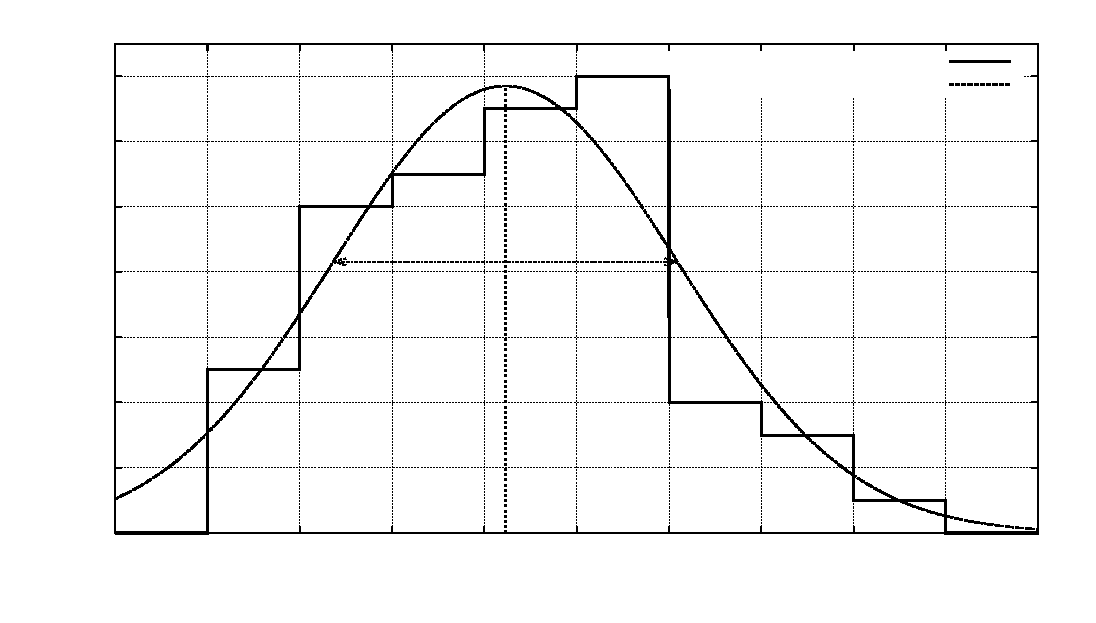
\includegraphics{hist}}%
    \gplfronttext
  \end{picture}%
\endgroup

\caption{Histogram rychlostí částic}
\label{g:hist}
\end{graph}

\begin{graph}[htbp] 
\centering
% GNUPLOT: LaTeX picture with Postscript
\begingroup
  \makeatletter
  \providecommand\color[2][]{%
    \GenericError{(gnuplot) \space\space\space\@spaces}{%
      Package color not loaded in conjunction with
      terminal option `colourtext'%
    }{See the gnuplot documentation for explanation.%
    }{Either use 'blacktext' in gnuplot or load the package
      color.sty in LaTeX.}%
    \renewcommand\color[2][]{}%
  }%
  \providecommand\includegraphics[2][]{%
    \GenericError{(gnuplot) \space\space\space\@spaces}{%
      Package graphicx or graphics not loaded%
    }{See the gnuplot documentation for explanation.%
    }{The gnuplot epslatex terminal needs graphicx.sty or graphics.sty.}%
    \renewcommand\includegraphics[2][]{}%
  }%
  \providecommand\rotatebox[2]{#2}%
  \@ifundefined{ifGPcolor}{%
    \newif\ifGPcolor
    \GPcolorfalse
  }{}%
  \@ifundefined{ifGPblacktext}{%
    \newif\ifGPblacktext
    \GPblacktexttrue
  }{}%
  % define a \g@addto@macro without @ in the name:
  \let\gplgaddtomacro\g@addto@macro
  % define empty templates for all commands taking text:
  \gdef\gplbacktext{}%
  \gdef\gplfronttext{}%
  \makeatother
  \ifGPblacktext
    % no textcolor at all
    \def\colorrgb#1{}%
    \def\colorgray#1{}%
  \else
    % gray or color?
    \ifGPcolor
      \def\colorrgb#1{\color[rgb]{#1}}%
      \def\colorgray#1{\color[gray]{#1}}%
      \expandafter\def\csname LTw\endcsname{\color{white}}%
      \expandafter\def\csname LTb\endcsname{\color{black}}%
      \expandafter\def\csname LTa\endcsname{\color{black}}%
      \expandafter\def\csname LT0\endcsname{\color[rgb]{1,0,0}}%
      \expandafter\def\csname LT1\endcsname{\color[rgb]{0,1,0}}%
      \expandafter\def\csname LT2\endcsname{\color[rgb]{0,0,1}}%
      \expandafter\def\csname LT3\endcsname{\color[rgb]{1,0,1}}%
      \expandafter\def\csname LT4\endcsname{\color[rgb]{0,1,1}}%
      \expandafter\def\csname LT5\endcsname{\color[rgb]{1,1,0}}%
      \expandafter\def\csname LT6\endcsname{\color[rgb]{0,0,0}}%
      \expandafter\def\csname LT7\endcsname{\color[rgb]{1,0.3,0}}%
      \expandafter\def\csname LT8\endcsname{\color[rgb]{0.5,0.5,0.5}}%
    \else
      % gray
      \def\colorrgb#1{\color{black}}%
      \def\colorgray#1{\color[gray]{#1}}%
      \expandafter\def\csname LTw\endcsname{\color{white}}%
      \expandafter\def\csname LTb\endcsname{\color{black}}%
      \expandafter\def\csname LTa\endcsname{\color{black}}%
      \expandafter\def\csname LT0\endcsname{\color{black}}%
      \expandafter\def\csname LT1\endcsname{\color{black}}%
      \expandafter\def\csname LT2\endcsname{\color{black}}%
      \expandafter\def\csname LT3\endcsname{\color{black}}%
      \expandafter\def\csname LT4\endcsname{\color{black}}%
      \expandafter\def\csname LT5\endcsname{\color{black}}%
      \expandafter\def\csname LT6\endcsname{\color{black}}%
      \expandafter\def\csname LT7\endcsname{\color{black}}%
      \expandafter\def\csname LT8\endcsname{\color{black}}%
    \fi
  \fi
  \setlength{\unitlength}{0.0500bp}%
  \begin{picture}(10204.00,4534.00)%
    \gplgaddtomacro\gplbacktext{%
      \csname LTb\endcsname%
      \put(396,484){\makebox(0,0){\strut{} 60}}%
      \put(1740,484){\makebox(0,0){\strut{} 65}}%
      \put(3085,484){\makebox(0,0){\strut{} 70}}%
      \put(4429,484){\makebox(0,0){\strut{} 75}}%
      \put(5774,484){\makebox(0,0){\strut{} 80}}%
      \put(7118,484){\makebox(0,0){\strut{} 85}}%
      \put(8463,484){\makebox(0,0){\strut{} 90}}%
      \put(9807,484){\makebox(0,0){\strut{} 95}}%
      \put(176,2486){\rotatebox{-270}{\makebox(0,0){\strut{}intenzita}}}%
      \put(5101,154){\makebox(0,0){\strut{}čas (\si{\ms})}}%
    }%
    \gplgaddtomacro\gplfronttext{%
    }%
    \gplbacktext
    \put(0,0){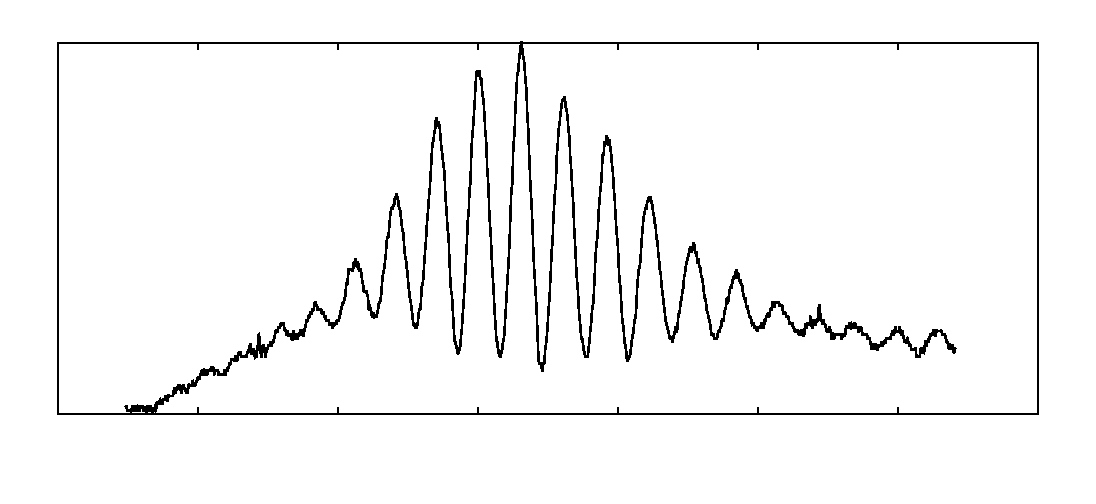
\includegraphics{typ}}%
    \gplfronttext
  \end{picture}%
\endgroup

\caption{Pozorovaný diferenciální dopplerovský signál}
\label{g:typ}
\end{graph}

%Diskuze výsledků
\section*{Diskuze}

%Závěr
\section*{Závěr}
Provedli jsme kalibraci "optické sondy anemometru" dvěma metodami. Obě metody daly téměř shodné výsledky, vzdálenost interferenčních plošek v průsečíku je
\begin{equation*}
d_F = \SI{29(1)}{\micro\m} \,.
\end{equation*}

Měření rychlosti částic bylo poněkud neúspěšné (viz diskuze). Histogram na první pohled neodpovídá normálnímu rozdělení. Určili jsme střední rychlost $\mu$ částic a standardní odchylku $\sigma$ rozdělení
\begin{align*}
\mu &= \SI{21.1(11)}{\mm\per\s}\\
\sigma &= \SI{9.3(12)}{\mm\per\s}
\end{align*}


\printbibliography[title={Seznam použité literatury}]

\end{document}